\documentclass[a4paper,11pt]{jsarticle}

% 数式
\usepackage{amsmath,amsfonts}
\usepackage{amsthm}
\usepackage{bm}
\usepackage{mathtools}
\usepackage{amssymb}

% 表
\usepackage[utf8]{inputenc}
\usepackage{diagbox} % 斜線付きセルを作成するために必要
\usepackage{booktabs} % 表の罫線を美しくするために必要
\usepackage{hhline} % 水平罫線を制御するために必要

% 画像
\usepackage[dvipdfmx]{graphicx}
\usepackage{ascmac}
\usepackage{physics}
\usepackage{float} % 追加

% 図
\usepackage[dvipdfmx]{graphicx}
\usepackage{tikz} %図を描く
\usetikzlibrary{positioning, intersections, calc, arrows.meta,math} %tikzのlibrary

% ハイパーリンク
\usepackage[dvipdfm,
  colorlinks=false,
  bookmarks=true,
  bookmarksnumbered=false,
  pdfborder={0 0 0},
  bookmarkstype=toc]{hyperref}

% 式番号を章ごとにリセット
\numberwithin{equation}{section}

\begin{document}

\title{効率とパワーのトレードオフ}
\author{大上由人}
\date{\today}
\maketitle

\section{エントロピー生成率の下限}
熱浴のエントロピー生成率は、
\begin{align}
  \theta_{j \to k}(t) &= \log(\frac{\omega_{j \to k}(t)}{\omega_{k \to j}(t)})\\
  &= \log(\frac{R_{kj}(t)}{R_{jk}(t)})
\end{align}
である。このとき、熱浴と系の全エントロピー生成は、
\begin{align}
  \sigma(t) &= \dv{t}S(\vb{p})(t) + \ev{\hat{\theta}(t)}_t 
\end{align}
である。ここで、$S(\vb{p})$は系のシャノンエントロピーであり、$\ev{\hat{\theta}(t)}_t$は時刻$t$における熱浴のエントロピー生成の期待値である。このとき、エントロピー生成の下限として、以下が知られている。
\begin{itembox}[l]{\textbf{Thm:エントロピー生成の下限}}
    エントロピー生成率は、以下の不等式を満たす:
    \begin{align}
      \sigma(t) \geq \sum_{j,k(j \neq k)}\frac{(R_{kj}(t)p_j(t)-R_{kj}(t)p_k(t))^2}{R_{kj}(t)P_j(t)+R_{jk}(t)P_k(t)} \geq 0
    \end{align}
    ただし、分子について、
    \begin{align}
      j_{j\to k}(t) &= R_{kj}(t)p_j(t)-R_{kj}(t)p_k(t)
    \end{align}
    である。
\end{itembox}
この式は、カレントがnonzeroであるとき、エントロピー生成がnonzeroになることを表している。

\textbf{Prf}\\
\begin{align}
    \dv{t}S(\vb{p}(t)) &= -\dv{t}\sum_k^{\Omega}p_k(t)\log p_k(t)\\
    &= -\sum_k^{\Omega}\dv{t}p_k(t)\log p_k(t) - \sum_k^{\Omega}p_k(t)\dv{t}\log p_k(t)\\
    &= -\sum_k^{\Omega}\dv{t}p_k(t)\log p_k(t) - \sum_k^{\Omega}\dv{t}p_k(t)\\
    &= -\sum_k^{\Omega}\dv{t}p_k(t)\log p_k(t)\quad (\because 規格化条件)\\
    &= -\sum_{j,k}^{\Omega}R_{kj}(t)p_j(t)\log p_j(t)\\
    &= \sum_{j,k}^{\Omega}R_{kj}(t)p_j(t)\log(\frac{p_j(t)}{p_k(t)}) \quad (\because \sum_{k}^{\Omega}R_{kj}(t) = 0)
\end{align}
である。また、
\begin{align}
    \ev{\hat{\theta}(t)}_t &= \sum_{j,k(j \neq k)}^{\Omega}R_{kj}(t)p_j(t)\log(\frac{R_{kj}(t)}{R_{jk}(t)})\\
    &= \sum_{j,k}^{\Omega}R_{kj}(t)p_j(t)\log(\frac{R_{kj}(t)p_j(t)}{R_{jk}(t)p_k(t)})\quad (\because \log 1 = 0)
\end{align}
である。これらを用いて、
\begin{align}
    \sigma(t) &= \dv{t}S(\vb{p}(t)) + \ev{\hat{\theta}(t)}_t\\
    &= \sum_{j,k}^{\Omega}R_{kj}(t)p_j(t)\log(\frac{R_{kj}(t)p_j(t)}{R_{jk}(t)p_k(t)}) \\
    &= \sum_{j,k(j \neq k)}^{\Omega}R_{kj}(t)p_j(t)\log(\frac{R_{kj}(t)p_j(t)}{R_{jk}(t)p_k(t)})\\
    &= \frac{1}{2}\sum_{j,k(j \neq k)}^{\Omega}\left(R_{kj}(t)p_j(t)-R_{jk}(t)p_k(t)\right)\log(\frac{R_{kj}(t)p_j(t)}{R_{jk}(t)p_k(t)}) \quad (\because \text{添え字に対する対称性})\\
    &\geq \sum_{j,k(j \neq k)}^{\Omega}\frac{(R_{kj}(t)p_j(t)-R_{jk}(t)p_k(t))^2}{2(R_{kj}(t)p_j(t)+R_{jk}(t)p_k(t))} \quad \left(\because \frac{1}{2}(a-b)\log(a/b) \geq \frac{(a-b)^2}{2(a+b)}\right)
\end{align}
である。よって示された。\qedsymbol

\section{Improved Shiraishi-Saito inequality}

$g_{j \to k}(t)$を、時刻$t$におけるjump quantityとし、
\begin{align}
  g_{j \to k}(t) = -g_{k \to j}(t) \quad (j \neq k)
\end{align}
とする。このとき、以下の不等式が成立する。

\begin{itembox}[l]{\textbf{Thm:Improved Shiraishi-Saito inequality}}
    jump quantityの平均値は、以下の不等式を満たす:
    \begin{align}
      |\ev{\hat{g}}_t| \leq \sqrt{\sigma(t)\Xi_g(t)}
    \end{align}
    ただし、$\sigma(t)$はエントロピー生成率であり、$\Xi_g(t)$は、
    \begin{align}
      \Xi_g(t) = \frac{1}{4} \sum_{j,k(j \neq k)}^{\Omega} (R_{kj}(t)p_j(t)+R_{jk}(t)p_k(t))g_{j \to k}(t)^2
    \end{align}
    である。


\end{itembox}
\textbf{Prf}\\
jump quantityの平均値は、
\begin{align}
  \ev{\hat{g}(t)}_t &= \sum_{j,k(j \neq k)}^{\Omega} p_j(t)\omega_{j \to k}(t)g_{j \to k}(t)\\
    &= \sum_{j,k(j \neq k)}^{\Omega} R_{kj}(t)p_j(t)g_{j \to k}(t)\\
    &= \frac{1}{2}\sum_{j,k(j \neq k)}^{\Omega} (R_{kj}(t)p_j(t)-R_{jk}(t)p_k(t))g_{j \to k}(t)\\
    &= \frac{1}{2}\sum_{j,k(j \neq k)}^{\Omega} (R_{kj}(t)p_j(t)-R_{jk}(t)p_k(t))g_{j \to k}(t) \quad (\because \text{添え字に対する対称性})\\
    &= \frac{1}{2}\sum_{j,k(j \neq k)}^{\Omega} \frac{R_{kj}(t)p_j(t)-R_{jk}(t)p_k(t)}{\sqrt{R_{kj}(t)p_j(t)+R_{jk}(t)p_k(t)}}\sqrt{R_{kj}(t)p_j(t)+R_{jk}(t)p_k(t)}g_{j \to k}(t)
\end{align}
である。ここで、Cauchy-Schwarzの不等式を用いると、
\begin{align}
    |\ev{\hat{g}}_t| &\leq \sqrt{\sum_{j,k(j \neq k)}^{\Omega} \frac{(R_{kj}(t)p_j(t)-R_{jk}(t)p_k(t))^2}{R_{kj}(t)p_j(t)+R_{jk}(t)p_k(t)} \cdot \frac{1}{4} \sum_{j,k(j \neq k)}^{\Omega} (R_{kj}(t)p_j(t)+R_{jk}(t)p_k(t))g_{j \to k}(t)^2}
\end{align}
である。ここで、第一項は$\sigma(t)$である。第二項を$\Xi_g(t)$とすると、
\begin{align}
  |\ev{\hat{g}}_t| &\leq \sqrt{\sigma(t)\Xi_g(t)}
\end{align}
である。よって示された。\qedsymbol\\

この不等式を変形することで、
\begin{align}
    \sigma(t) \geq \frac{|\ev{\hat{g}}_t|^2}{\Xi_g(t)}
\end{align}
となる。これは、jump quantityの平均値がnonzeroであるとき、エントロピー生成がnonzeroになることを表している。\\

このとき、
\begin{align}
    \Xi_g(t) &= \frac{1}{4}\sum_{j,k(j \neq k)}^{\Omega}(R_{kj}(t)p_j(t)+R_{jk}(t)p_k(t))g_{j \to k}(t)^2\\
    &= \frac{1}{2}\sum_{j,k(j \neq k)}^{\Omega}(R_{kj}(t)p_j(t))g_{j \to k}(t)^2
\end{align}
は一般には有限であることが知られている。とくに、jump quantityが有限かつ、escape rateが有限であるとき、すなわち、
\begin{align}
    |g_{j \to k}(t)| \leq g_0 ,\quad \lambda_j \leq \lambda_0
\end{align}
であるとき、
\begin{align}
    \Xi_g(t) \leq \frac{1}{2}g_0^2\lambda_0
\end{align}
である。

得られた不等式を変形すると、
\begin{align}
    \sigma(t) \geq \frac{|\ev{\hat{g}}_t|^2}{\Xi_g(t)}
\end{align}
である。これは、jump quantityの平均値がnonzeroであるとき、エントロピー生成率がnonzeroになることを表している。

また、時間平均をとることで、以下の不等式が成り立つことが知られている。
\begin{itembox}[l]{\textbf{Thm:Improved Shiraishi-Saito inequality(時間平均)}}
    jump quantityの時間平均値は、以下の不等式を満たす:
    \begin{align}
      \overline{\Xi}_g ^{-1}\qty(\lim_{\tau \to \infty}\frac{1}{\tau}\int_0^{\tau} \dd{t}\ev{\hat{g}}_t)^2 \leq \lim_{\tau \to \infty}\frac{1}{\tau}\int_0^{\tau} \dd{t}\ev{\hat{\theta}_t}_t
    \end{align}
    ただし、$\overline{\Xi_g}$は、
    \begin{align}
      \overline{\Xi}_g = \lim_{\tau \to \infty}\frac{1}{\tau}\int_0^{\tau} \dd{t}\Xi_g(t)
    \end{align}
    である。

\end{itembox}
\textbf{Prf}\\
普通のShiraishi-Saito不等式より、
\begin{align}
  \ev{\hat{g}}_t \leq \sqrt{\sigma(t)\Xi_g(t)}
\end{align}
である。Cauchy-Schwarzの不等式より、
\begin{align}
  \frac{1}{\tau}\int_0^{\tau} \dd{t}\ev{\hat{g}(t)}_t \leq \sqrt{\frac{1}{\tau}\int_0^{\tau} \dd{t}\sigma(t) \frac{1}{\tau}\int_0^{\tau} \dd{t} \Xi_g(t)}
\end{align}
である。ところで、
\begin{align}
  \frac{1}{\tau}\int_0^{\tau} \dd{t}\ev{\sigma(t)}_t &= \frac{1}{\tau}(S(\vb{p}(\tau)) - S(\vb{p}(0))) + \frac{1}{\tau}\int_0^{\tau} \dd{t}\ev{\hat{\theta}(t)}_t
\end{align}
である。この右辺第一項は、$\tau \to \infty$で、$S(\vb{p}(\tau)) - S(\vb{p}(0)) \to 0$である。よって、
\begin{align}
  \frac{1}{\tau}\int_0^{\tau} \dd{t}\ev{g(t)}_t \leq \sqrt{\lim_{\tau \to \infty}\frac{1}{\tau}\int_0^{\tau} \dd{t}\ev{\hat{\theta(t)}}_t \overline{\Xi}_g}
\end{align}
である。よって示された。\qedsymbol\\

この不等式は、jump quantityの平均値がnonzeroであるとき、(カレントがnonzeroであるとき)平均の(熱浴での)散逸がnonzeroになることを表している。\\
ここで、長時間平均によりShanonエントロピーの項が消えることは重要である。というのも、シャノンエントロピーを知るためには粒子のミクロな状態を知らなくてはならないが、実際問題それが難しいためである。

\section{熱機関の、パワーと効率のトレードオフ}
\textbf{設定}\\
\begin{figure}[H]
    \begin{center}
    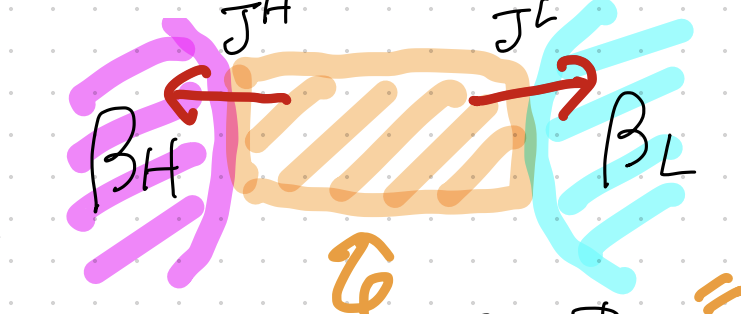
\includegraphics[width=100mm]{set.png}
    \end{center}
    \caption{設定}
    \label{fig:set}
\end{figure}

系が二つの熱浴に接触しているとする。$\alpha = \text{H,L}$で、それぞれの熱浴の逆温度を$\beta_{\alpha}$、遷移レートを$\omega_{j \to k}(t)$、系のエネルギーを$E_j(t)$とする。このとき、局所詳細釣り合い条件は、
\begin{align}
  \log \frac{\omega_{j \to k}(t)}{\omega_{k \to j}(t)} = \beta_{\alpha(j,k)}(E_j(t) - E_k(t))
\end{align}
である。($\alpha(j,k) = \text{H,L}$)\\
熱浴への熱の流れは、
\begin{align}
  {J}^{\alpha}_{j\to k}(t) =
  \begin{cases}
    E_j(t) - E_k(t) & \alpha(j,k) = \alpha\\
    0 & \text{otherwise}
    \end{cases}
\end{align}
である。また、エントロピー生成は、
\begin{align}
  \theta_{j \to k}(t) & \beta_{\alpha(j,k)}(E_j(t) - E_k(t))\\
    &= \beta_{\text{H}}J^{\text{H}}_{j\to k}(t) + \beta_{\text{L}}J^{\text{L}}_{j\to k}(t)
\end{align}
である。
\textbf{仮定}\\
\begin{figure}[H]
    \begin{center}
    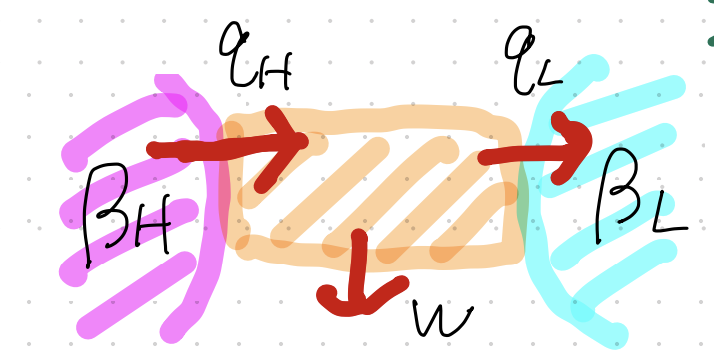
\includegraphics[width=100mm]{set2.png}
    \end{center}
    \caption{仮定}
    \label{fig:set2}
\end{figure}

以下の極限が存在し、その極限値が正であるとする:
\begin{align}
  q_H &= -\lim_{\tau \to \infty}\frac{1}{\tau}\int_0^{\tau} \dd{t}\ev{\hat{J}^H(t)}_t>0\\
  q_L &= \lim_{\tau \to \infty}\frac{1}{\tau}\int_0^{\tau} \dd{t}\ev{\hat{J}^L(t)}_t>0
\end{align}
これは、高温熱浴から系に入ってくる熱流および、低温熱浴に流れる熱流の時間平均である。また、このとき、平均のパワー(仕事率)は、
\begin{align}
  W = q_H - q_L
\end{align}
であり、効率は、
\begin{align}
  \eta = \frac{W}{q_H} = 1 - \frac{q_L}{q_H}
\end{align}
である。このとき、以下の不等式が成立する。

\begin{itembox}[l]{\textbf{Thm:熱機関の、パワーと効率のトレードオフ}}
    熱機関のパワーと効率は、以下の不等式を満たす:
    \begin{align}
      (q_H + q_L)^2 \leq \overline{\Xi} \beta_L q_H (\eta_{\text{C}} - \eta) 
    \end{align}

\end{itembox}
\textbf{Prf}\\
今、
\begin{align}
    \lim_{\tau \to \infty}\frac{1}{\tau}\int_0^{\tau} \dd{t}\ev{\hat{\theta}_t}_t &= -\beta_H q_H + \beta_L q_L\\
    &= -\beta_H q_H + \beta_L (q_H - W)\\
    &= \beta_L q_H \qty(-\frac{\beta_H}{\beta_L} + 1 - \frac{W}{q_H})\\
      &= \beta_L q_H (\eta_{\text{C}} - \eta) (\geq 0)
  \end{align}
  である。また、
\begin{align}
  g_{j \to k}(t) = \hat{J}_{j \to k}^L(t) - \hat{J}_{j \to k}^H(t)
\end{align}
とする。このとき、Shiraishi-Saito不等式より、
\begin{align}
  \left(\frac{1}{\tau}\int_0^{\tau} \dd{t}\ev{\hat{g}(t)}_t\right)^2 \leq \overline{\Xi} \lim_{\tau \to \infty}\frac{1}{\tau}\int_0^{\tau} \dd{t}\ev{\hat{\theta}_t}_t
\end{align}
である。ここで、
\begin{align}
  \overline{\Xi} = \lim_{\tau \to \infty}\frac{1}{\tau} \dd{t} \frac{1}{2}\sum_{j,k(j \neq k)}^{\Omega} R_{kj}(t)p_j(t) (E_j(t) - E_k(t))^2
\end{align}
である。(これは、どれくらいactiveに熱のやり取りをするかを表している。)このとき、
\begin{align}
  \qty(\frac{1}{\tau}\int_0^{\tau} \dd{t}\ev{\hat{g}(t)}_t)^2 = (q_H + q_L)^2
\end{align}
である。よって、
\begin{align}
  (q_H + q_L)^2 \leq \overline{\Xi} \beta_L q_H (\eta_{\text{C}} - \eta)
\end{align}
である。よって示された。\qedsymbol\\

上で得られた不等式を変形すると、
\begin{align}
  \overline{\Xi} \beta_L(\eta_{\text{C}} - \eta) \geq \frac{(q_H + q_L)^2}{q_H} \geq q_H + q_L
\end{align}
となる。これは、効率がカルノーサイクルに近づくと、$q_H, q_L$が0に近づくことを表している。このもとで、パワーは0に近づくことがわかる。\\
あるいは、以下のようにも変形できる:
\begin{align}
  W &\leq \overline{\Xi} \beta_L\frac{q_H}{(q_H + q_L)^2}(\eta_{\text{C}} - \eta)W\\
  &= \overline{\Xi} \beta_L\frac{q_H}{(q_H + q_L)^2}\eta(\eta_{\text{C}} - \eta)\quad (\because W = q_H \eta)\\
    &\leq \overline{\Xi} \beta_L\eta(\eta_{\text{C}} - \eta)
\end{align}
これは、効率がカルノーサイクルに近づくと、パワーが0に近づくことを直接的に示している。\\

\end{document}